\documentclass[1p]{elsarticle_modified}
%\bibliographystyle{elsarticle-num}

%\usepackage[colorlinks]{hyperref}
%\usepackage{abbrmath_seonhwa} %\Abb, \Ascr, \Acal ,\Abf, \Afrak
\usepackage{amsfonts}
\usepackage{amssymb}
\usepackage{amsmath}
\usepackage{amsthm}
\usepackage{scalefnt}
\usepackage{amsbsy}
\usepackage{kotex}
\usepackage{caption}
\usepackage{subfig}
\usepackage{color}
\usepackage{graphicx}
\usepackage{xcolor} %% white, black, red, green, blue, cyan, magenta, yellow
\usepackage{float}
\usepackage{setspace}
\usepackage{hyperref}

\usepackage{tikz}
\usetikzlibrary{arrows}

\usepackage{multirow}
\usepackage{array} % fixed length table
\usepackage{hhline}

%%%%%%%%%%%%%%%%%%%%%
\makeatletter
\renewcommand*\env@matrix[1][\arraystretch]{%
	\edef\arraystretch{#1}%
	\hskip -\arraycolsep
	\let\@ifnextchar\new@ifnextchar
	\array{*\c@MaxMatrixCols c}}
\makeatother %https://tex.stackexchange.com/questions/14071/how-can-i-increase-the-line-spacing-in-a-matrix
%%%%%%%%%%%%%%%

\usepackage[normalem]{ulem}

\newcommand{\msout}[1]{\ifmmode\text{\sout{\ensuremath{#1}}}\else\sout{#1}\fi}
%SOURCE: \msout is \stkout macro in https://tex.stackexchange.com/questions/20609/strikeout-in-math-mode

\newcommand{\cancel}[1]{
	\ifmmode
	{\color{red}\msout{#1}}
	\else
	{\color{red}\sout{#1}}
	\fi
}

\newcommand{\add}[1]{
	{\color{blue}\uwave{#1}}
}

\newcommand{\replace}[2]{
	\ifmmode
	{\color{red}\msout{#1}}{\color{blue}\uwave{#2}}
	\else
	{\color{red}\sout{#1}}{\color{blue}\uwave{#2}}
	\fi
}

\newcommand{\Sol}{\mathcal{S}} %segment
\newcommand{\D}{D} %diagram
\newcommand{\A}{\mathcal{A}} %arc


%%%%%%%%%%%%%%%%%%%%%%%%%%%%%5 test

\def\sl{\operatorname{\textup{SL}}(2,\Cbb)}
\def\psl{\operatorname{\textup{PSL}}(2,\Cbb)}
\def\quan{\mkern 1mu \triangleright \mkern 1mu}

\theoremstyle{definition}
\newtheorem{thm}{Theorem}[section]
\newtheorem{prop}[thm]{Proposition}
\newtheorem{lem}[thm]{Lemma}
\newtheorem{ques}[thm]{Question}
\newtheorem{cor}[thm]{Corollary}
\newtheorem{defn}[thm]{Definition}
\newtheorem{exam}[thm]{Example}
\newtheorem{rmk}[thm]{Remark}
\newtheorem{alg}[thm]{Algorithm}

\newcommand{\I}{\sqrt{-1}}
\begin{document}

%\begin{frontmatter}
%
%\title{Boundary parabolic representations of knots up to 8 crossings}
%
%%% Group authors per affiliation:
%\author{Yunhi Cho} 
%\address{Department of Mathematics, University of Seoul, Seoul, Korea}
%\ead{yhcho@uos.ac.kr}
%
%
%\author{Seonhwa Kim} %\fnref{s_kim}}
%\address{Center for Geometry and Physics, Institute for Basic Science, Pohang, 37673, Korea}
%\ead{ryeona17@ibs.re.kr}
%
%\author{Hyuk Kim}
%\address{Department of Mathematical Sciences, Seoul National University, Seoul 08826, Korea}
%\ead{hyukkim@snu.ac.kr}
%
%\author{Seokbeom Yoon}
%\address{Department of Mathematical Sciences, Seoul National University, Seoul, 08826,  Korea}
%\ead{sbyoon15@snu.ac.kr}
%
%\begin{abstract}
%We find all boundary parabolic representation of knots up to 8 crossings.
%
%\end{abstract}
%\begin{keyword}
%    \MSC[2010] 57M25 
%\end{keyword}
%
%\end{frontmatter}

%\linenumbers
%\tableofcontents
%
\newcommand\colored[1]{\textcolor{white}{\rule[-0.35ex]{0.8em}{1.4ex}}\kern-0.8em\color{red} #1}%
%\newcommand\colored[1]{\textcolor{white}{ #1}\kern-2.17ex	\textcolor{white}{ #1}\kern-1.81ex	\textcolor{white}{ #1}\kern-2.15ex\color{red}#1	}

{\Large $\underline{12n_{0646}~(K12n_{0646})}$}

\setlength{\tabcolsep}{10pt}
\renewcommand{\arraystretch}{1.6}
\vspace{1cm}\begin{tabular}{m{100pt}>{\centering\arraybackslash}m{274pt}}
\multirow{5}{120pt}{
	\centering
	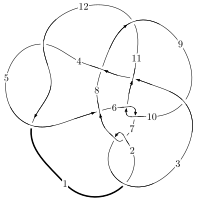
\includegraphics[width=112pt]{../../../GIT/diagram.site/Diagrams/png/2735_12n_0646.png}\\
\ \ \ A knot diagram\footnotemark}&
\allowdisplaybreaks
\textbf{Linearized knot diagam} \\
\cline{2-2}
 &
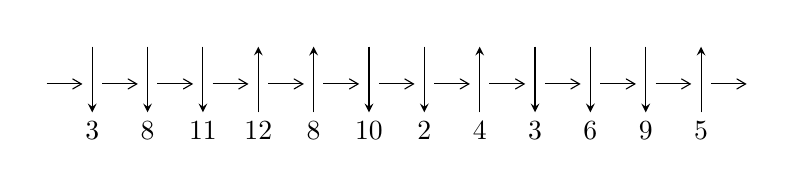
\begin{tikzpicture}[x=20pt, y=17pt]
	% nodes
	\node (C0) at (0, 0) {};
	\node (C1) at (1, 0) {};
	\node (C1U) at (1, +1) {};
	\node (C1D) at (1, -1) {3};

	\node (C2) at (2, 0) {};
	\node (C2U) at (2, +1) {};
	\node (C2D) at (2, -1) {8};

	\node (C3) at (3, 0) {};
	\node (C3U) at (3, +1) {};
	\node (C3D) at (3, -1) {11};

	\node (C4) at (4, 0) {};
	\node (C4U) at (4, +1) {};
	\node (C4D) at (4, -1) {12};

	\node (C5) at (5, 0) {};
	\node (C5U) at (5, +1) {};
	\node (C5D) at (5, -1) {8};

	\node (C6) at (6, 0) {};
	\node (C6U) at (6, +1) {};
	\node (C6D) at (6, -1) {10};

	\node (C7) at (7, 0) {};
	\node (C7U) at (7, +1) {};
	\node (C7D) at (7, -1) {2};

	\node (C8) at (8, 0) {};
	\node (C8U) at (8, +1) {};
	\node (C8D) at (8, -1) {4};

	\node (C9) at (9, 0) {};
	\node (C9U) at (9, +1) {};
	\node (C9D) at (9, -1) {3};

	\node (C10) at (10, 0) {};
	\node (C10U) at (10, +1) {};
	\node (C10D) at (10, -1) {6};

	\node (C11) at (11, 0) {};
	\node (C11U) at (11, +1) {};
	\node (C11D) at (11, -1) {9};

	\node (C12) at (12, 0) {};
	\node (C12U) at (12, +1) {};
	\node (C12D) at (12, -1) {5};
	\node (C13) at (13, 0) {};

	% arrows
	\draw[->,>={angle 60}]
	(C0) edge (C1) (C1) edge (C2) (C2) edge (C3) (C3) edge (C4) (C4) edge (C5) (C5) edge (C6) (C6) edge (C7) (C7) edge (C8) (C8) edge (C9) (C9) edge (C10) (C10) edge (C11) (C11) edge (C12) (C12) edge (C13) ;	\draw[->,>=stealth]
	(C1U) edge (C1D) (C2U) edge (C2D) (C3U) edge (C3D) (C4D) edge (C4U) (C5D) edge (C5U) (C6U) edge (C6D) (C7U) edge (C7D) (C8D) edge (C8U) (C9U) edge (C9D) (C10U) edge (C10D) (C11U) edge (C11D) (C12D) edge (C12U) ;
	\end{tikzpicture} \\
\hhline{~~} \\& 
\textbf{Solving Sequence} \\ \cline{2-2} 
 &
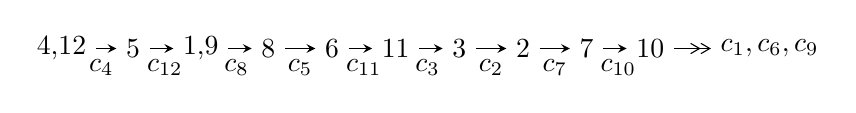
\begin{tikzpicture}[x=23pt, y=7pt]
	% node
	\node (A0) at (-1/8, 0) {4,12};
	\node (A1) at (1, 0) {5};
	\node (A2) at (33/16, 0) {1,9};
	\node (A3) at (25/8, 0) {8};
	\node (A4) at (33/8, 0) {6};
	\node (A5) at (41/8, 0) {11};
	\node (A6) at (49/8, 0) {3};
	\node (A7) at (57/8, 0) {2};
	\node (A8) at (65/8, 0) {7};
	\node (A9) at (73/8, 0) {10};
	\node (C1) at (1/2, -1) {$c_{4}$};
	\node (C2) at (3/2, -1) {$c_{12}$};
	\node (C3) at (21/8, -1) {$c_{8}$};
	\node (C4) at (29/8, -1) {$c_{5}$};
	\node (C5) at (37/8, -1) {$c_{11}$};
	\node (C6) at (45/8, -1) {$c_{3}$};
	\node (C7) at (53/8, -1) {$c_{2}$};
	\node (C8) at (61/8, -1) {$c_{7}$};
	\node (C9) at (69/8, -1) {$c_{10}$};
	\node (A10) at (11, 0) {$c_{1},c_{6},c_{9}$};

	% edge
	\draw[->,>=stealth]	
	(A0) edge (A1) (A1) edge (A2) (A2) edge (A3) (A3) edge (A4) (A4) edge (A5) (A5) edge (A6) (A6) edge (A7) (A7) edge (A8) (A8) edge (A9) ;
	\draw[->>,>={angle 60}]	
	(A9) edge (A10);
\end{tikzpicture} \\ 

\end{tabular} \\

\footnotetext{
The image of knot diagram is generated by the software ``\textbf{Draw programme}" developed by Andrew Bartholomew(\url{http://www.layer8.co.uk/maths/draw/index.htm\#Running-draw}), where we modified some parts for our purpose(\url{https://github.com/CATsTAILs/LinksPainter}).
}\phantom \\ \newline 
\centering \textbf{Ideals for irreducible components\footnotemark of $X_{\text{par}}$} 
 
\begin{align*}
I^u_{1}&=\langle 
1.58803\times10^{237} u^{73}+9.98357\times10^{236} u^{72}+\cdots+1.04871\times10^{239} b-4.84351\times10^{239},\\
\phantom{I^u_{1}}&\phantom{= \langle  }2.36054\times10^{238} u^{73}+1.15336\times10^{239} u^{72}+\cdots+6.18737\times10^{240} a+6.07876\times10^{241},\\
\phantom{I^u_{1}}&\phantom{= \langle  }u^{74}-23 u^{72}+\cdots-1348 u+59\rangle \\
I^u_{2}&=\langle 
10945 u^{22}+124117 u^{21}+\cdots+323513 b-770040,\\
\phantom{I^u_{2}}&\phantom{= \langle  }-1292813 u^{22}-1139926 u^{21}+\cdots+2264591 a-1752915,\;u^{23}+u^{22}+\cdots+6 u+7\rangle \\
\\
\end{align*}
\raggedright * 2 irreducible components of $\dim_{\mathbb{C}}=0$, with total 97 representations.\\
\footnotetext{All coefficients of polynomials are rational numbers. But the coefficients are sometimes approximated in decimal forms when there is not enough margin.}
\newpage
\renewcommand{\arraystretch}{1}
\centering \section*{I. $I^u_{1}= \langle 1.59\times10^{237} u^{73}+9.98\times10^{236} u^{72}+\cdots+1.05\times10^{239} b-4.84\times10^{239},\;2.36\times10^{238} u^{73}+1.15\times10^{239} u^{72}+\cdots+6.19\times10^{240} a+6.08\times10^{241},\;u^{74}-23 u^{72}+\cdots-1348 u+59 \rangle$}
\flushleft \textbf{(i) Arc colorings}\\
\begin{tabular}{m{7pt} m{180pt} m{7pt} m{180pt} }
\flushright $a_{4}=$&$\begin{pmatrix}1\\0\end{pmatrix}$ \\
\flushright $a_{12}=$&$\begin{pmatrix}0\\u\end{pmatrix}$ \\
\flushright $a_{5}=$&$\begin{pmatrix}1\\- u^2\end{pmatrix}$ \\
\flushright $a_{1}=$&$\begin{pmatrix}u\\- u^3+u\end{pmatrix}$ \\
\flushright $a_{9}=$&$\begin{pmatrix}-0.00381509 u^{73}-0.0186406 u^{72}+\cdots+143.928 u-9.82446\\-0.0151427 u^{73}-0.00951988 u^{72}+\cdots-57.5931 u+4.61855\end{pmatrix}$ \\
\flushright $a_{8}=$&$\begin{pmatrix}0.0113276 u^{73}-0.00912068 u^{72}+\cdots+201.521 u-14.4430\\-0.0151427 u^{73}-0.00951988 u^{72}+\cdots-57.5931 u+4.61855\end{pmatrix}$ \\
\flushright $a_{6}=$&$\begin{pmatrix}0.0317970 u^{73}+0.0254113 u^{72}+\cdots+41.9592 u-9.10400\\-0.0151377 u^{73}-0.0157835 u^{72}+\cdots+8.09941 u-0.430016\end{pmatrix}$ \\
\flushright $a_{11}=$&$\begin{pmatrix}-0.0232878 u^{73}-0.0230889 u^{72}+\cdots+5.49692 u-4.11660\\0.0139050 u^{73}+0.00829155 u^{72}+\cdots+29.1837 u-0.868546\end{pmatrix}$ \\
\flushright $a_{3}=$&$\begin{pmatrix}-0.0319762 u^{73}-0.0216255 u^{72}+\cdots-71.9715 u+6.77566\\0.0246533 u^{73}+0.0189372 u^{72}+\cdots+32.4888 u-1.70516\end{pmatrix}$ \\
\flushright $a_{2}=$&$\begin{pmatrix}0.0124870 u^{73}+0.0121558 u^{72}+\cdots+18.8902 u-1.56877\\-0.0138331 u^{73}-0.0119768 u^{72}+\cdots-19.0668 u+0.944486\end{pmatrix}$ \\
\flushright $a_{7}=$&$\begin{pmatrix}-0.0344961 u^{73}-0.0473584 u^{72}+\cdots+140.483 u-11.9122\\0.0110322 u^{73}+0.0116464 u^{72}+\cdots-18.3283 u+2.94677\end{pmatrix}$ \\
\flushright $a_{10}=$&$\begin{pmatrix}-0.0361091 u^{73}-0.0518980 u^{72}+\cdots+169.740 u-14.6086\\0.0250197 u^{73}+0.0231141 u^{72}+\cdots-2.04277 u+2.76319\end{pmatrix}$\\&\end{tabular}
\flushleft \textbf{(ii) Obstruction class $= -1$}\\~\\
\flushleft \textbf{(iii) Cusp Shapes $= -0.00383692 u^{73}+0.0116603 u^{72}+\cdots-82.4847 u+0.241670$}\\~\\
\newpage\renewcommand{\arraystretch}{1}
\flushleft \textbf{(iv) u-Polynomials at the component}\newline \\
\begin{tabular}{m{50pt}|m{274pt}}
Crossings & \hspace{64pt}u-Polynomials at each crossing \\
\hline $$\begin{aligned}c_{1}\end{aligned}$$&$\begin{aligned}
&u^{74}+83 u^{73}+\cdots-742961 u+32761
\end{aligned}$\\
\hline $$\begin{aligned}c_{2},c_{7}\end{aligned}$$&$\begin{aligned}
&u^{74}+u^{73}+\cdots-1071 u+181
\end{aligned}$\\
\hline $$\begin{aligned}c_{3}\end{aligned}$$&$\begin{aligned}
&u^{74}+5 u^{73}+\cdots+35 u+67
\end{aligned}$\\
\hline $$\begin{aligned}c_{4},c_{12}\end{aligned}$$&$\begin{aligned}
&u^{74}-23 u^{72}+\cdots-1348 u+59
\end{aligned}$\\
\hline $$\begin{aligned}c_{5}\end{aligned}$$&$\begin{aligned}
&u^{74}+12 u^{73}+\cdots+241794036 u+20549479
\end{aligned}$\\
\hline $$\begin{aligned}c_{6},c_{10}\end{aligned}$$&$\begin{aligned}
&u^{74}+9 u^{72}+\cdots+14 u+1
\end{aligned}$\\
\hline $$\begin{aligned}c_{8}\end{aligned}$$&$\begin{aligned}
&u^{74}-3 u^{73}+\cdots+9 u-1
\end{aligned}$\\
\hline $$\begin{aligned}c_{9}\end{aligned}$$&$\begin{aligned}
&u^{74}- u^{73}+\cdots+5432040 u-294541
\end{aligned}$\\
\hline $$\begin{aligned}c_{11}\end{aligned}$$&$\begin{aligned}
&u^{74}- u^{73}+\cdots+26 u-1
\end{aligned}$\\
\hline
\end{tabular}\\~\\
\newpage\renewcommand{\arraystretch}{1}
\flushleft \textbf{(v) Riley Polynomials at the component}\newline \\
\begin{tabular}{m{50pt}|m{274pt}}
Crossings & \hspace{64pt}Riley Polynomials at each crossing \\
\hline $$\begin{aligned}c_{1}\end{aligned}$$&$\begin{aligned}
&y^{74}-171 y^{73}+\cdots-248386801315 y+1073283121
\end{aligned}$\\
\hline $$\begin{aligned}c_{2},c_{7}\end{aligned}$$&$\begin{aligned}
&y^{74}-83 y^{73}+\cdots+742961 y+32761
\end{aligned}$\\
\hline $$\begin{aligned}c_{3}\end{aligned}$$&$\begin{aligned}
&y^{74}-23 y^{73}+\cdots-170601 y+4489
\end{aligned}$\\
\hline $$\begin{aligned}c_{4},c_{12}\end{aligned}$$&$\begin{aligned}
&y^{74}-46 y^{73}+\cdots-867912 y+3481
\end{aligned}$\\
\hline $$\begin{aligned}c_{5}\end{aligned}$$&$\begin{aligned}
&y^{74}+72 y^{73}+\cdots+4872087324166162 y+422281087171441
\end{aligned}$\\
\hline $$\begin{aligned}c_{6},c_{10}\end{aligned}$$&$\begin{aligned}
&y^{74}+18 y^{73}+\cdots-460 y+1
\end{aligned}$\\
\hline $$\begin{aligned}c_{8}\end{aligned}$$&$\begin{aligned}
&y^{74}-9 y^{73}+\cdots-129 y+1
\end{aligned}$\\
\hline $$\begin{aligned}c_{9}\end{aligned}$$&$\begin{aligned}
&y^{74}-41 y^{73}+\cdots-4467923151064 y+86754400681
\end{aligned}$\\
\hline $$\begin{aligned}c_{11}\end{aligned}$$&$\begin{aligned}
&y^{74}+7 y^{73}+\cdots-144 y+1
\end{aligned}$\\
\hline
\end{tabular}\\~\\
\newpage\flushleft \textbf{(vi) Complex Volumes and Cusp Shapes}
$$\begin{array}{c|c|c}  
\text{Solutions to }I^u_{1}& \I (\text{vol} + \sqrt{-1}CS) & \text{Cusp shape}\\
 \hline 
\begin{aligned}
u &= -0.655798 + 0.766408 I \\
a &= \phantom{-}0.869120 + 0.744224 I \\
b &= -1.35513 + 0.70847 I\end{aligned}
 & -8.29346 + 2.75368 I & \phantom{-0.000000 } 0 \\ \hline\begin{aligned}
u &= -0.655798 - 0.766408 I \\
a &= \phantom{-}0.869120 - 0.744224 I \\
b &= -1.35513 - 0.70847 I\end{aligned}
 & -8.29346 - 2.75368 I & \phantom{-0.000000 } 0 \\ \hline\begin{aligned}
u &= -0.965313 + 0.158931 I \\
a &= \phantom{-}0.972971 - 0.580114 I \\
b &= -0.574458 + 0.287498 I\end{aligned}
 & \phantom{-}1.82145 - 4.11786 I & \phantom{-0.000000 -}0. + 8.23328 I \\ \hline\begin{aligned}
u &= -0.965313 - 0.158931 I \\
a &= \phantom{-}0.972971 + 0.580114 I \\
b &= -0.574458 - 0.287498 I\end{aligned}
 & \phantom{-}1.82145 + 4.11786 I & \phantom{-0.000000 } 0. - 8.23328 I \\ \hline\begin{aligned}
u &= -0.915463 + 0.481248 I \\
a &= -1.301600 - 0.360841 I \\
b &= \phantom{-}1.42148 - 0.29716 I\end{aligned}
 & -7.16001 - 3.26958 I & \phantom{-0.000000 } 0 \\ \hline\begin{aligned}
u &= -0.915463 - 0.481248 I \\
a &= -1.301600 + 0.360841 I \\
b &= \phantom{-}1.42148 + 0.29716 I\end{aligned}
 & -7.16001 + 3.26958 I & \phantom{-0.000000 } 0 \\ \hline\begin{aligned}
u &= -0.846052 + 0.596785 I \\
a &= -0.148846 - 0.608636 I \\
b &= -1.10293 - 1.17110 I\end{aligned}
 & -7.32108 - 1.01128 I & \phantom{-0.000000 } 0 \\ \hline\begin{aligned}
u &= -0.846052 - 0.596785 I \\
a &= -0.148846 + 0.608636 I \\
b &= -1.10293 + 1.17110 I\end{aligned}
 & -7.32108 + 1.01128 I & \phantom{-0.000000 } 0 \\ \hline\begin{aligned}
u &= -0.964557 + 0.396965 I \\
a &= -0.392535 - 1.170080 I \\
b &= \phantom{-}1.22014 - 1.00039 I\end{aligned}
 & \phantom{-}1.18006 - 5.95366 I & \phantom{-0.000000 } 0 \\ \hline\begin{aligned}
u &= -0.964557 - 0.396965 I \\
a &= -0.392535 + 1.170080 I \\
b &= \phantom{-}1.22014 + 1.00039 I\end{aligned}
 & \phantom{-}1.18006 + 5.95366 I & \phantom{-0.000000 } 0\\
 \hline 
 \end{array}$$\newpage$$\begin{array}{c|c|c}  
\text{Solutions to }I^u_{1}& \I (\text{vol} + \sqrt{-1}CS) & \text{Cusp shape}\\
 \hline 
\begin{aligned}
u &= \phantom{-}0.985961 + 0.412954 I \\
a &= -2.13540 - 0.84349 I \\
b &= \phantom{-}0.367620 + 0.144013 I\end{aligned}
 & -5.83823 + 6.62476 I & \phantom{-0.000000 } 0 \\ \hline\begin{aligned}
u &= \phantom{-}0.985961 - 0.412954 I \\
a &= -2.13540 + 0.84349 I \\
b &= \phantom{-}0.367620 - 0.144013 I\end{aligned}
 & -5.83823 - 6.62476 I & \phantom{-0.000000 } 0 \\ \hline\begin{aligned}
u &= \phantom{-}0.774737 + 0.472773 I \\
a &= \phantom{-}0.78398 + 1.88499 I \\
b &= -0.437396 + 0.860845 I\end{aligned}
 & -6.51675 - 3.02533 I & -7.09255 + 5.00598 I \\ \hline\begin{aligned}
u &= \phantom{-}0.774737 - 0.472773 I \\
a &= \phantom{-}0.78398 - 1.88499 I \\
b &= -0.437396 - 0.860845 I\end{aligned}
 & -6.51675 + 3.02533 I & -7.09255 - 5.00598 I \\ \hline\begin{aligned}
u &= -0.894325\phantom{ +0.000000I} \\
a &= -1.14517\phantom{ +0.000000I} \\
b &= \phantom{-}0.120420\phantom{ +0.000000I}\end{aligned}
 & -0.954299\phantom{ +0.000000I} & -9.82620\phantom{ +0.000000I} \\ \hline\begin{aligned}
u &= \phantom{-}0.021010 + 0.882929 I \\
a &= -0.855935 - 0.904683 I \\
b &= -0.535620 - 0.743252 I\end{aligned}
 & -2.26108 + 2.43230 I & -9.75705 - 2.77573 I \\ \hline\begin{aligned}
u &= \phantom{-}0.021010 - 0.882929 I \\
a &= -0.855935 + 0.904683 I \\
b &= -0.535620 + 0.743252 I\end{aligned}
 & -2.26108 - 2.43230 I & -9.75705 + 2.77573 I \\ \hline\begin{aligned}
u &= \phantom{-}0.753306 + 0.428451 I \\
a &= -0.01914 + 1.95753 I \\
b &= \phantom{-}0.815160 + 0.718326 I\end{aligned}
 & \phantom{-}2.81045 + 5.61623 I & -4.20124 - 6.00638 I \\ \hline\begin{aligned}
u &= \phantom{-}0.753306 - 0.428451 I \\
a &= -0.01914 - 1.95753 I \\
b &= \phantom{-}0.815160 - 0.718326 I\end{aligned}
 & \phantom{-}2.81045 - 5.61623 I & -4.20124 + 6.00638 I \\ \hline\begin{aligned}
u &= \phantom{-}0.845381 + 0.156772 I \\
a &= -0.179363 + 0.806483 I \\
b &= \phantom{-}0.937521 + 0.034650 I\end{aligned}
 & \phantom{-}2.50679 + 0.22280 I & \phantom{-}1.160362 - 0.536343 I\\
 \hline 
 \end{array}$$\newpage$$\begin{array}{c|c|c}  
\text{Solutions to }I^u_{1}& \I (\text{vol} + \sqrt{-1}CS) & \text{Cusp shape}\\
 \hline 
\begin{aligned}
u &= \phantom{-}0.845381 - 0.156772 I \\
a &= -0.179363 - 0.806483 I \\
b &= \phantom{-}0.937521 - 0.034650 I\end{aligned}
 & \phantom{-}2.50679 - 0.22280 I & \phantom{-}1.160362 + 0.536343 I \\ \hline\begin{aligned}
u &= -0.747820 + 0.348453 I \\
a &= \phantom{-}0.02740 - 1.73267 I \\
b &= \phantom{-}0.281766 - 0.913256 I\end{aligned}
 & -1.09279 - 2.96806 I & -12.4081 + 9.2557 I \\ \hline\begin{aligned}
u &= -0.747820 - 0.348453 I \\
a &= \phantom{-}0.02740 + 1.73267 I \\
b &= \phantom{-}0.281766 + 0.913256 I\end{aligned}
 & -1.09279 + 2.96806 I & -12.4081 - 9.2557 I \\ \hline\begin{aligned}
u &= \phantom{-}1.097690 + 0.464463 I \\
a &= -0.09607 - 1.62484 I \\
b &= \phantom{-}0.098368 - 0.983912 I\end{aligned}
 & -6.21900 + 4.81585 I & \phantom{-0.000000 } 0 \\ \hline\begin{aligned}
u &= \phantom{-}1.097690 - 0.464463 I \\
a &= -0.09607 + 1.62484 I \\
b &= \phantom{-}0.098368 + 0.983912 I\end{aligned}
 & -6.21900 - 4.81585 I & \phantom{-0.000000 } 0 \\ \hline\begin{aligned}
u &= -1.049620 + 0.578940 I \\
a &= \phantom{-}0.147679 + 0.427039 I \\
b &= \phantom{-}0.92680 + 1.54482 I\end{aligned}
 & -7.02322 - 7.85025 I & \phantom{-0.000000 } 0 \\ \hline\begin{aligned}
u &= -1.049620 - 0.578940 I \\
a &= \phantom{-}0.147679 - 0.427039 I \\
b &= \phantom{-}0.92680 - 1.54482 I\end{aligned}
 & -7.02322 + 7.85025 I & \phantom{-0.000000 } 0 \\ \hline\begin{aligned}
u &= -1.202410 + 0.158541 I \\
a &= \phantom{-}0.089960 + 0.140257 I \\
b &= -0.784654 - 0.680195 I\end{aligned}
 & \phantom{-}1.55515 + 3.70197 I & \phantom{-0.000000 } 0 \\ \hline\begin{aligned}
u &= -1.202410 - 0.158541 I \\
a &= \phantom{-}0.089960 - 0.140257 I \\
b &= -0.784654 + 0.680195 I\end{aligned}
 & \phantom{-}1.55515 - 3.70197 I & \phantom{-0.000000 } 0 \\ \hline\begin{aligned}
u &= \phantom{-}0.771268 + 0.039152 I \\
a &= \phantom{-}0.981686 - 0.957054 I \\
b &= -1.49247 - 0.58340 I\end{aligned}
 & \phantom{-}1.74698 + 0.32926 I & -1.62591 + 0.32056 I\\
 \hline 
 \end{array}$$\newpage$$\begin{array}{c|c|c}  
\text{Solutions to }I^u_{1}& \I (\text{vol} + \sqrt{-1}CS) & \text{Cusp shape}\\
 \hline 
\begin{aligned}
u &= \phantom{-}0.771268 - 0.039152 I \\
a &= \phantom{-}0.981686 + 0.957054 I \\
b &= -1.49247 + 0.58340 I\end{aligned}
 & \phantom{-}1.74698 - 0.32926 I & -1.62591 - 0.32056 I \\ \hline\begin{aligned}
u &= \phantom{-}0.919006 + 0.821173 I \\
a &= -0.192595 + 0.795743 I \\
b &= \phantom{-}1.17685 + 0.91692 I\end{aligned}
 & \phantom{-}1.35546 + 3.43403 I & \phantom{-0.000000 } 0 \\ \hline\begin{aligned}
u &= \phantom{-}0.919006 - 0.821173 I \\
a &= -0.192595 - 0.795743 I \\
b &= \phantom{-}1.17685 - 0.91692 I\end{aligned}
 & \phantom{-}1.35546 - 3.43403 I & \phantom{-0.000000 } 0 \\ \hline\begin{aligned}
u &= -1.243770 + 0.270809 I \\
a &= \phantom{-}0.596369 + 1.181910 I \\
b &= -0.997710 + 0.666984 I\end{aligned}
 & \phantom{-}6.67491 - 4.74644 I & \phantom{-0.000000 } 0 \\ \hline\begin{aligned}
u &= -1.243770 - 0.270809 I \\
a &= \phantom{-}0.596369 - 1.181910 I \\
b &= -0.997710 - 0.666984 I\end{aligned}
 & \phantom{-}6.67491 + 4.74644 I & \phantom{-0.000000 } 0 \\ \hline\begin{aligned}
u &= \phantom{-}0.470959 + 0.537045 I \\
a &= \phantom{-}2.62151 - 1.11038 I \\
b &= -0.046697 - 0.372483 I\end{aligned}
 & -8.14386 - 0.75783 I & -15.9338 - 3.9359 I \\ \hline\begin{aligned}
u &= \phantom{-}0.470959 - 0.537045 I \\
a &= \phantom{-}2.62151 + 1.11038 I \\
b &= -0.046697 + 0.372483 I\end{aligned}
 & -8.14386 + 0.75783 I & -15.9338 + 3.9359 I \\ \hline\begin{aligned}
u &= \phantom{-}1.282620 + 0.200693 I \\
a &= \phantom{-}0.554347 - 0.664419 I \\
b &= -1.40018 - 1.15063 I\end{aligned}
 & \phantom{-}2.91081 + 4.20783 I & \phantom{-0.000000 } 0 \\ \hline\begin{aligned}
u &= \phantom{-}1.282620 - 0.200693 I \\
a &= \phantom{-}0.554347 + 0.664419 I \\
b &= -1.40018 + 1.15063 I\end{aligned}
 & \phantom{-}2.91081 - 4.20783 I & \phantom{-0.000000 } 0 \\ \hline\begin{aligned}
u &= -1.298030 + 0.205140 I \\
a &= -0.432301 - 1.003540 I \\
b &= \phantom{-}1.09376 - 1.17630 I\end{aligned}
 & \phantom{-}1.90861 - 6.12809 I & \phantom{-0.000000 } 0\\
 \hline 
 \end{array}$$\newpage$$\begin{array}{c|c|c}  
\text{Solutions to }I^u_{1}& \I (\text{vol} + \sqrt{-1}CS) & \text{Cusp shape}\\
 \hline 
\begin{aligned}
u &= -1.298030 - 0.205140 I \\
a &= -0.432301 + 1.003540 I \\
b &= \phantom{-}1.09376 + 1.17630 I\end{aligned}
 & \phantom{-}1.90861 + 6.12809 I & \phantom{-0.000000 } 0 \\ \hline\begin{aligned}
u &= \phantom{-}1.312430 + 0.246619 I \\
a &= -0.159546 + 0.445122 I \\
b &= \phantom{-}0.847012 + 0.717184 I\end{aligned}
 & \phantom{-}2.74861 + 1.42952 I & \phantom{-0.000000 } 0 \\ \hline\begin{aligned}
u &= \phantom{-}1.312430 - 0.246619 I \\
a &= -0.159546 - 0.445122 I \\
b &= \phantom{-}0.847012 - 0.717184 I\end{aligned}
 & \phantom{-}2.74861 - 1.42952 I & \phantom{-0.000000 } 0 \\ \hline\begin{aligned}
u &= -0.328781 + 1.323690 I \\
a &= \phantom{-}0.348126 + 0.339963 I \\
b &= \phantom{-}0.525286 + 0.880984 I\end{aligned}
 & -1.14232 + 4.08189 I & \phantom{-0.000000 } 0 \\ \hline\begin{aligned}
u &= -0.328781 - 1.323690 I \\
a &= \phantom{-}0.348126 - 0.339963 I \\
b &= \phantom{-}0.525286 - 0.880984 I\end{aligned}
 & -1.14232 - 4.08189 I & \phantom{-0.000000 } 0 \\ \hline\begin{aligned}
u &= \phantom{-}0.396021 + 0.484207 I \\
a &= -0.478537 + 0.330222 I \\
b &= -0.14607 + 1.42484 I\end{aligned}
 & -1.06612 + 2.28791 I & -9.94456 - 3.29711 I \\ \hline\begin{aligned}
u &= \phantom{-}0.396021 - 0.484207 I \\
a &= -0.478537 - 0.330222 I \\
b &= -0.14607 - 1.42484 I\end{aligned}
 & -1.06612 - 2.28791 I & -9.94456 + 3.29711 I \\ \hline\begin{aligned}
u &= -0.378716 + 0.457118 I \\
a &= \phantom{-}1.64287 - 0.19150 I \\
b &= \phantom{-}0.780151 - 0.056187 I\end{aligned}
 & \phantom{-}3.34314 + 2.04546 I & -1.45171 - 1.17441 I \\ \hline\begin{aligned}
u &= -0.378716 - 0.457118 I \\
a &= \phantom{-}1.64287 + 0.19150 I \\
b &= \phantom{-}0.780151 + 0.056187 I\end{aligned}
 & \phantom{-}3.34314 - 2.04546 I & -1.45171 + 1.17441 I \\ \hline\begin{aligned}
u &= -1.23386 + 0.70848 I \\
a &= \phantom{-}0.298842 + 0.935259 I \\
b &= -1.27459 + 1.00051 I\end{aligned}
 & \phantom{-}1.59205 - 10.86400 I & \phantom{-0.000000 } 0\\
 \hline 
 \end{array}$$\newpage$$\begin{array}{c|c|c}  
\text{Solutions to }I^u_{1}& \I (\text{vol} + \sqrt{-1}CS) & \text{Cusp shape}\\
 \hline 
\begin{aligned}
u &= -1.23386 - 0.70848 I \\
a &= \phantom{-}0.298842 - 0.935259 I \\
b &= -1.27459 - 1.00051 I\end{aligned}
 & \phantom{-}1.59205 + 10.86400 I & \phantom{-0.000000 } 0 \\ \hline\begin{aligned}
u &= \phantom{-}1.39427 + 0.45022 I \\
a &= -0.240132 - 0.502315 I \\
b &= -0.452753 - 0.074158 I\end{aligned}
 & \phantom{-}4.81856 - 1.48237 I & \phantom{-0.000000 } 0 \\ \hline\begin{aligned}
u &= \phantom{-}1.39427 - 0.45022 I \\
a &= -0.240132 + 0.502315 I \\
b &= -0.452753 + 0.074158 I\end{aligned}
 & \phantom{-}4.81856 + 1.48237 I & \phantom{-0.000000 } 0 \\ \hline\begin{aligned}
u &= -1.47129\phantom{ +0.000000I} \\
a &= -0.811222\phantom{ +0.000000I} \\
b &= \phantom{-}0.288330\phantom{ +0.000000I}\end{aligned}
 & -1.54712\phantom{ +0.000000I} & \phantom{-0.000000 } 0 \\ \hline\begin{aligned}
u &= \phantom{-}1.43434 + 0.38897 I \\
a &= -0.540506 + 0.537467 I \\
b &= \phantom{-}1.36368 + 0.82268 I\end{aligned}
 & \phantom{-}2.16075 + 2.17644 I & \phantom{-0.000000 } 0 \\ \hline\begin{aligned}
u &= \phantom{-}1.43434 - 0.38897 I \\
a &= -0.540506 - 0.537467 I \\
b &= \phantom{-}1.36368 - 0.82268 I\end{aligned}
 & \phantom{-}2.16075 - 2.17644 I & \phantom{-0.000000 } 0 \\ \hline\begin{aligned}
u &= \phantom{-}0.11140 + 1.48650 I \\
a &= -0.446418 + 0.632857 I \\
b &= -0.726218 + 0.933179 I\end{aligned}
 & -10.06450 - 9.11027 I & \phantom{-0.000000 } 0 \\ \hline\begin{aligned}
u &= \phantom{-}0.11140 - 1.48650 I \\
a &= -0.446418 - 0.632857 I \\
b &= -0.726218 - 0.933179 I\end{aligned}
 & -10.06450 + 9.11027 I & \phantom{-0.000000 } 0 \\ \hline\begin{aligned}
u &= \phantom{-}1.27797 + 0.77796 I \\
a &= \phantom{-}0.054128 - 0.537788 I \\
b &= -0.661480 - 0.188312 I\end{aligned}
 & \phantom{-}2.27044 + 3.86617 I & \phantom{-0.000000 } 0 \\ \hline\begin{aligned}
u &= \phantom{-}1.27797 - 0.77796 I \\
a &= \phantom{-}0.054128 + 0.537788 I \\
b &= -0.661480 + 0.188312 I\end{aligned}
 & \phantom{-}2.27044 - 3.86617 I & \phantom{-0.000000 } 0\\
 \hline 
 \end{array}$$\newpage$$\begin{array}{c|c|c}  
\text{Solutions to }I^u_{1}& \I (\text{vol} + \sqrt{-1}CS) & \text{Cusp shape}\\
 \hline 
\begin{aligned}
u &= \phantom{-}0.50265 + 1.41427 I \\
a &= \phantom{-}0.552978 - 0.455848 I \\
b &= \phantom{-}0.585875 - 0.772913 I\end{aligned}
 & -9.71632 - 1.35291 I & \phantom{-0.000000 } 0 \\ \hline\begin{aligned}
u &= \phantom{-}0.50265 - 1.41427 I \\
a &= \phantom{-}0.552978 + 0.455848 I \\
b &= \phantom{-}0.585875 + 0.772913 I\end{aligned}
 & -9.71632 + 1.35291 I & \phantom{-0.000000 } 0 \\ \hline\begin{aligned}
u &= \phantom{-}1.26097 + 0.83176 I \\
a &= \phantom{-}0.199374 - 1.092040 I \\
b &= -1.05828 - 1.03852 I\end{aligned}
 & -7.22130 + 8.96738 I & \phantom{-0.000000 } 0 \\ \hline\begin{aligned}
u &= \phantom{-}1.26097 - 0.83176 I \\
a &= \phantom{-}0.199374 + 1.092040 I \\
b &= -1.05828 + 1.03852 I\end{aligned}
 & -7.22130 - 8.96738 I & \phantom{-0.000000 } 0 \\ \hline\begin{aligned}
u &= -0.478233\phantom{ +0.000000I} \\
a &= -1.48533\phantom{ +0.000000I} \\
b &= -0.193213\phantom{ +0.000000I}\end{aligned}
 & -1.01756\phantom{ +0.000000I} & -9.85560\phantom{ +0.000000I} \\ \hline\begin{aligned}
u &= \phantom{-}1.44910 + 0.71346 I \\
a &= -0.339147 + 0.994028 I \\
b &= \phantom{-}1.20794 + 1.04725 I\end{aligned}
 & -5.8720 + 16.6158 I & \phantom{-0.000000 } 0 \\ \hline\begin{aligned}
u &= \phantom{-}1.44910 - 0.71346 I \\
a &= -0.339147 - 0.994028 I \\
b &= \phantom{-}1.20794 - 1.04725 I\end{aligned}
 & -5.8720 - 16.6158 I & \phantom{-0.000000 } 0 \\ \hline\begin{aligned}
u &= -1.43999 + 0.91289 I \\
a &= \phantom{-}0.078936 - 0.637578 I \\
b &= \phantom{-}0.840470 - 0.448062 I\end{aligned}
 & -3.71000 - 8.50390 I & \phantom{-0.000000 } 0 \\ \hline\begin{aligned}
u &= -1.43999 - 0.91289 I \\
a &= \phantom{-}0.078936 + 0.637578 I \\
b &= \phantom{-}0.840470 + 0.448062 I\end{aligned}
 & -3.71000 + 8.50390 I & \phantom{-0.000000 } 0 \\ \hline\begin{aligned}
u &= -1.20485 + 1.21909 I \\
a &= -0.197169 + 0.455659 I \\
b &= -0.678604 + 0.449090 I\end{aligned}
 & -5.22524 - 0.83630 I & \phantom{-0.000000 } 0\\
 \hline 
 \end{array}$$\newpage$$\begin{array}{c|c|c}  
\text{Solutions to }I^u_{1}& \I (\text{vol} + \sqrt{-1}CS) & \text{Cusp shape}\\
 \hline 
\begin{aligned}
u &= -1.20485 - 1.21909 I \\
a &= -0.197169 - 0.455659 I \\
b &= -0.678604 - 0.449090 I\end{aligned}
 & -5.22524 + 0.83630 I & \phantom{-0.000000 } 0 \\ \hline\begin{aligned}
u &= \phantom{-}0.0777028 + 0.0283731 I \\
a &= \phantom{-}2.71739 + 4.75753 I \\
b &= \phantom{-}0.447185 - 1.220730 I\end{aligned}
 & -0.88271 - 2.35880 I & -7.30268 - 2.94254 I \\ \hline\begin{aligned}
u &= \phantom{-}0.0777028 - 0.0283731 I \\
a &= \phantom{-}2.71739 - 4.75753 I \\
b &= \phantom{-}0.447185 + 1.220730 I\end{aligned}
 & -0.88271 + 2.35880 I & -7.30268 + 2.94254 I \\ \hline\begin{aligned}
u &= -2.48363\phantom{ +0.000000I} \\
a &= \phantom{-}0.0328074\phantom{ +0.000000I} \\
b &= \phantom{-}0.360820\phantom{ +0.000000I}\end{aligned}
 & -2.98919\phantom{ +0.000000I} & \phantom{-0.000000 } 0\\
 \hline 
 \end{array}$$\newpage\newpage\renewcommand{\arraystretch}{1}
\centering \section*{II. $I^u_{2}= \langle 1.09\times10^{4} u^{22}+1.24\times10^{5} u^{21}+\cdots+3.24\times10^{5} b-7.70\times10^{5},\;-1.29\times10^{6} u^{22}-1.14\times10^{6} u^{21}+\cdots+2.26\times10^{6} a-1.75\times10^{6},\;u^{23}+u^{22}+\cdots+6 u+7 \rangle$}
\flushleft \textbf{(i) Arc colorings}\\
\begin{tabular}{m{7pt} m{180pt} m{7pt} m{180pt} }
\flushright $a_{4}=$&$\begin{pmatrix}1\\0\end{pmatrix}$ \\
\flushright $a_{12}=$&$\begin{pmatrix}0\\u\end{pmatrix}$ \\
\flushright $a_{5}=$&$\begin{pmatrix}1\\- u^2\end{pmatrix}$ \\
\flushright $a_{1}=$&$\begin{pmatrix}u\\- u^3+u\end{pmatrix}$ \\
\flushright $a_{9}=$&$\begin{pmatrix}0.570881 u^{22}+0.503369 u^{21}+\cdots+0.996580 u+0.774054\\-0.0338317 u^{22}-0.383654 u^{21}+\cdots+4.19368 u+2.38024\end{pmatrix}$ \\
\flushright $a_{8}=$&$\begin{pmatrix}0.604713 u^{22}+0.887023 u^{21}+\cdots-3.19710 u-1.60619\\-0.0338317 u^{22}-0.383654 u^{21}+\cdots+4.19368 u+2.38024\end{pmatrix}$ \\
\flushright $a_{6}=$&$\begin{pmatrix}0.715072 u^{22}+1.60066 u^{21}+\cdots-8.26166 u-0.692739\\0.140643 u^{22}+0.0151895 u^{21}+\cdots+3.15600 u+2.81671\end{pmatrix}$ \\
\flushright $a_{11}=$&$\begin{pmatrix}-0.174507 u^{22}-1.00570 u^{21}+\cdots+6.80089 u+5.50371\\0.444573 u^{22}+0.348014 u^{21}+\cdots-3.73106 u+0.847542\end{pmatrix}$ \\
\flushright $a_{3}=$&$\begin{pmatrix}-0.741805 u^{22}-0.369258 u^{21}+\cdots-2.84354 u-2.11154\\0.00713109 u^{22}+0.988770 u^{21}+\cdots-3.38884 u-3.70637\end{pmatrix}$ \\
\flushright $a_{2}=$&$\begin{pmatrix}-1.32743 u^{22}-0.253648 u^{21}+\cdots-5.63410 u-1.62524\\-0.143311 u^{22}+0.692522 u^{21}+\cdots-1.19043 u-3.87800\end{pmatrix}$ \\
\flushright $a_{7}=$&$\begin{pmatrix}-0.448108 u^{22}-0.0775385 u^{21}+\cdots-5.26590 u-2.41661\\-0.00353927 u^{22}-0.180382 u^{21}+\cdots+5.47344 u+2.04846\end{pmatrix}$ \\
\flushright $a_{10}=$&$\begin{pmatrix}-0.274671 u^{22}+0.497193 u^{21}+\cdots+4.96111 u-2.93448\\-0.0900397 u^{22}-0.245724 u^{21}+\cdots+1.23296 u+2.27996\end{pmatrix}$\\&\end{tabular}
\flushleft \textbf{(ii) Obstruction class $= 1$}\\~\\
\flushleft \textbf{(iii) Cusp Shapes $= \frac{116070}{323513} u^{22}-\frac{673312}{323513} u^{21}+\cdots+\frac{8778130}{323513} u+\frac{3192863}{323513}$}\\~\\
\newpage\renewcommand{\arraystretch}{1}
\flushleft \textbf{(iv) u-Polynomials at the component}\newline \\
\begin{tabular}{m{50pt}|m{274pt}}
Crossings & \hspace{64pt}u-Polynomials at each crossing \\
\hline $$\begin{aligned}c_{1}\end{aligned}$$&$\begin{aligned}
&u^{23}-22 u^{22}+\cdots+13 u-1
\end{aligned}$\\
\hline $$\begin{aligned}c_{2}\end{aligned}$$&$\begin{aligned}
&u^{23}-11 u^{21}+\cdots+3 u-1
\end{aligned}$\\
\hline $$\begin{aligned}c_{3}\end{aligned}$$&$\begin{aligned}
&u^{23}-5 u^{21}+\cdots- u+1
\end{aligned}$\\
\hline $$\begin{aligned}c_{4}\end{aligned}$$&$\begin{aligned}
&u^{23}+u^{22}+\cdots+6 u+7
\end{aligned}$\\
\hline $$\begin{aligned}c_{5}\end{aligned}$$&$\begin{aligned}
&u^{23}+u^{22}+\cdots-214 u-19
\end{aligned}$\\
\hline $$\begin{aligned}c_{6}\end{aligned}$$&$\begin{aligned}
&u^{23}+u^{22}+\cdots-2 u+1
\end{aligned}$\\
\hline $$\begin{aligned}c_{7}\end{aligned}$$&$\begin{aligned}
&u^{23}-11 u^{21}+\cdots+3 u+1
\end{aligned}$\\
\hline $$\begin{aligned}c_{8}\end{aligned}$$&$\begin{aligned}
&u^{23}-2 u^{21}+\cdots+3 u-1
\end{aligned}$\\
\hline $$\begin{aligned}c_{9}\end{aligned}$$&$\begin{aligned}
&u^{23}-4 u^{21}+\cdots-130 u+77
\end{aligned}$\\
\hline $$\begin{aligned}c_{10}\end{aligned}$$&$\begin{aligned}
&u^{23}- u^{22}+\cdots-2 u-1
\end{aligned}$\\
\hline $$\begin{aligned}c_{11}\end{aligned}$$&$\begin{aligned}
&u^{23}+4 u^{21}+\cdots+2 u-1
\end{aligned}$\\
\hline $$\begin{aligned}c_{12}\end{aligned}$$&$\begin{aligned}
&u^{23}- u^{22}+\cdots+6 u-7
\end{aligned}$\\
\hline
\end{tabular}\\~\\
\newpage\renewcommand{\arraystretch}{1}
\flushleft \textbf{(v) Riley Polynomials at the component}\newline \\
\begin{tabular}{m{50pt}|m{274pt}}
Crossings & \hspace{64pt}Riley Polynomials at each crossing \\
\hline $$\begin{aligned}c_{1}\end{aligned}$$&$\begin{aligned}
&y^{23}-30 y^{22}+\cdots-39 y-1
\end{aligned}$\\
\hline $$\begin{aligned}c_{2},c_{7}\end{aligned}$$&$\begin{aligned}
&y^{23}-22 y^{22}+\cdots+13 y-1
\end{aligned}$\\
\hline $$\begin{aligned}c_{3}\end{aligned}$$&$\begin{aligned}
&y^{23}-10 y^{22}+\cdots+11 y-1
\end{aligned}$\\
\hline $$\begin{aligned}c_{4},c_{12}\end{aligned}$$&$\begin{aligned}
&y^{23}-25 y^{22}+\cdots+414 y-49
\end{aligned}$\\
\hline $$\begin{aligned}c_{5}\end{aligned}$$&$\begin{aligned}
&y^{23}+9 y^{22}+\cdots-7860 y-361
\end{aligned}$\\
\hline $$\begin{aligned}c_{6},c_{10}\end{aligned}$$&$\begin{aligned}
&y^{23}+15 y^{22}+\cdots-22 y-1
\end{aligned}$\\
\hline $$\begin{aligned}c_{8}\end{aligned}$$&$\begin{aligned}
&y^{23}-4 y^{22}+\cdots+31 y-1
\end{aligned}$\\
\hline $$\begin{aligned}c_{9}\end{aligned}$$&$\begin{aligned}
&y^{23}-8 y^{22}+\cdots+27526 y-5929
\end{aligned}$\\
\hline $$\begin{aligned}c_{11}\end{aligned}$$&$\begin{aligned}
&y^{23}+8 y^{22}+\cdots-6 y-1
\end{aligned}$\\
\hline
\end{tabular}\\~\\
\newpage\flushleft \textbf{(vi) Complex Volumes and Cusp Shapes}
$$\begin{array}{c|c|c}  
\text{Solutions to }I^u_{2}& \I (\text{vol} + \sqrt{-1}CS) & \text{Cusp shape}\\
 \hline 
\begin{aligned}
u &= -0.940151 + 0.436724 I \\
a &= \phantom{-}1.38542 - 1.03904 I \\
b &= -0.375096 - 0.652275 I\end{aligned}
 & -6.14502 - 6.06691 I & -7.76620 + 2.70001 I \\ \hline\begin{aligned}
u &= -0.940151 - 0.436724 I \\
a &= \phantom{-}1.38542 + 1.03904 I \\
b &= -0.375096 + 0.652275 I\end{aligned}
 & -6.14502 + 6.06691 I & -7.76620 - 2.70001 I \\ \hline\begin{aligned}
u &= -0.899734 + 0.566100 I \\
a &= \phantom{-}0.666138 - 0.686902 I \\
b &= \phantom{-}0.587866 + 0.237361 I\end{aligned}
 & \phantom{-}3.26577 + 3.29082 I & \phantom{-}1.12702 - 5.35953 I \\ \hline\begin{aligned}
u &= -0.899734 - 0.566100 I \\
a &= \phantom{-}0.666138 + 0.686902 I \\
b &= \phantom{-}0.587866 - 0.237361 I\end{aligned}
 & \phantom{-}3.26577 - 3.29082 I & \phantom{-}1.12702 + 5.35953 I \\ \hline\begin{aligned}
u &= \phantom{-}1.167050 + 0.232734 I \\
a &= -0.746928 + 1.034470 I \\
b &= \phantom{-}1.145920 + 0.467030 I\end{aligned}
 & \phantom{-}5.42529 + 3.86107 I & \phantom{-}0.38428 - 3.23578 I \\ \hline\begin{aligned}
u &= \phantom{-}1.167050 - 0.232734 I \\
a &= -0.746928 - 1.034470 I \\
b &= \phantom{-}1.145920 - 0.467030 I\end{aligned}
 & \phantom{-}5.42529 - 3.86107 I & \phantom{-}0.38428 + 3.23578 I \\ \hline\begin{aligned}
u &= -0.193140 + 0.771651 I \\
a &= -0.749439 - 0.320841 I \\
b &= -0.598832 - 0.904838 I\end{aligned}
 & -0.70593 + 3.60670 I & -4.29911 - 3.93608 I \\ \hline\begin{aligned}
u &= -0.193140 - 0.771651 I \\
a &= -0.749439 + 0.320841 I \\
b &= -0.598832 + 0.904838 I\end{aligned}
 & -0.70593 - 3.60670 I & -4.29911 + 3.93608 I \\ \hline\begin{aligned}
u &= -1.203350 + 0.187731 I \\
a &= \phantom{-}0.50630 + 1.32809 I \\
b &= -0.956631 + 0.862062 I\end{aligned}
 & \phantom{-}4.95788 - 5.88075 I & -0.13221 + 5.80716 I \\ \hline\begin{aligned}
u &= -1.203350 - 0.187731 I \\
a &= \phantom{-}0.50630 - 1.32809 I \\
b &= -0.956631 - 0.862062 I\end{aligned}
 & \phantom{-}4.95788 + 5.88075 I & -0.13221 - 5.80716 I\\
 \hline 
 \end{array}$$\newpage$$\begin{array}{c|c|c}  
\text{Solutions to }I^u_{2}& \I (\text{vol} + \sqrt{-1}CS) & \text{Cusp shape}\\
 \hline 
\begin{aligned}
u &= \phantom{-}1.154040 + 0.447461 I \\
a &= -0.362840 - 0.500105 I \\
b &= -0.706629 - 0.294864 I\end{aligned}
 & \phantom{-}4.63415 - 0.90682 I & \phantom{-}1.28962 - 4.52518 I \\ \hline\begin{aligned}
u &= \phantom{-}1.154040 - 0.447461 I \\
a &= -0.362840 + 0.500105 I \\
b &= -0.706629 + 0.294864 I\end{aligned}
 & \phantom{-}4.63415 + 0.90682 I & \phantom{-}1.28962 + 4.52518 I \\ \hline\begin{aligned}
u &= -1.280170 + 0.173459 I \\
a &= -0.442367 - 0.893767 I \\
b &= \phantom{-}1.23555 - 1.29461 I\end{aligned}
 & \phantom{-}2.71445 - 6.27245 I & \phantom{-}2.92402 + 8.05584 I \\ \hline\begin{aligned}
u &= -1.280170 - 0.173459 I \\
a &= -0.442367 + 0.893767 I \\
b &= \phantom{-}1.23555 + 1.29461 I\end{aligned}
 & \phantom{-}2.71445 + 6.27245 I & \phantom{-}2.92402 - 8.05584 I \\ \hline\begin{aligned}
u &= \phantom{-}0.637930 + 0.249825 I \\
a &= -0.023201 - 1.259190 I \\
b &= -0.400551 - 1.237650 I\end{aligned}
 & -0.49072 + 2.75096 I & \phantom{-}2.90356 - 6.14599 I \\ \hline\begin{aligned}
u &= \phantom{-}0.637930 - 0.249825 I \\
a &= -0.023201 + 1.259190 I \\
b &= -0.400551 + 1.237650 I\end{aligned}
 & -0.49072 - 2.75096 I & \phantom{-}2.90356 + 6.14599 I \\ \hline\begin{aligned}
u &= -0.430937 + 0.491432 I \\
a &= -1.97377 - 0.90570 I \\
b &= \phantom{-}0.716053 + 0.206167 I\end{aligned}
 & -7.54393 + 1.02790 I & -3.87032 - 0.83091 I \\ \hline\begin{aligned}
u &= -0.430937 - 0.491432 I \\
a &= -1.97377 + 0.90570 I \\
b &= \phantom{-}0.716053 - 0.206167 I\end{aligned}
 & -7.54393 - 1.02790 I & -3.87032 + 0.83091 I \\ \hline\begin{aligned}
u &= \phantom{-}1.361540 + 0.157735 I \\
a &= -0.127050 + 0.265071 I \\
b &= \phantom{-}0.941423 + 0.657717 I\end{aligned}
 & \phantom{-}3.28773 + 2.35398 I & \phantom{-}1.50757 - 4.79947 I \\ \hline\begin{aligned}
u &= \phantom{-}1.361540 - 0.157735 I \\
a &= -0.127050 - 0.265071 I \\
b &= \phantom{-}0.941423 - 0.657717 I\end{aligned}
 & \phantom{-}3.28773 - 2.35398 I & \phantom{-}1.50757 + 4.79947 I\\
 \hline 
 \end{array}$$\newpage$$\begin{array}{c|c|c}  
\text{Solutions to }I^u_{2}& \I (\text{vol} + \sqrt{-1}CS) & \text{Cusp shape}\\
 \hline 
\begin{aligned}
u &= \phantom{-}1.307310 + 0.445348 I \\
a &= \phantom{-}0.501766 - 0.593735 I \\
b &= -1.48600 - 0.92539 I\end{aligned}
 & \phantom{-}2.02704 + 2.55701 I & -2.41189 - 10.60905 I \\ \hline\begin{aligned}
u &= \phantom{-}1.307310 - 0.445348 I \\
a &= \phantom{-}0.501766 + 0.593735 I \\
b &= -1.48600 + 0.92539 I\end{aligned}
 & \phantom{-}2.02704 - 2.55701 I & -2.41189 + 10.60905 I \\ \hline\begin{aligned}
u &= -2.36076\phantom{ +0.000000I} \\
a &= \phantom{-}0.160525\phantom{ +0.000000I} \\
b &= -0.206162\phantom{ +0.000000I}\end{aligned}
 & -3.11418\phantom{ +0.000000I} & -34.3130\phantom{ +0.000000I}\\
 \hline 
 \end{array}$$\newpage
\newpage\renewcommand{\arraystretch}{1}
\centering \section*{ III. u-Polynomials}
\begin{tabular}{m{50pt}|m{274pt}}
Crossings & \hspace{64pt}u-Polynomials at each crossing \\
\hline $$\begin{aligned}c_{1}\end{aligned}$$&$\begin{aligned}
&(u^{23}-22 u^{22}+\cdots+13 u-1)(u^{74}+83 u^{73}+\cdots-742961 u+32761)
\end{aligned}$\\
\hline $$\begin{aligned}c_{2}\end{aligned}$$&$\begin{aligned}
&(u^{23}-11 u^{21}+\cdots+3 u-1)(u^{74}+u^{73}+\cdots-1071 u+181)
\end{aligned}$\\
\hline $$\begin{aligned}c_{3}\end{aligned}$$&$\begin{aligned}
&(u^{23}-5 u^{21}+\cdots- u+1)(u^{74}+5 u^{73}+\cdots+35 u+67)
\end{aligned}$\\
\hline $$\begin{aligned}c_{4}\end{aligned}$$&$\begin{aligned}
&(u^{23}+u^{22}+\cdots+6 u+7)(u^{74}-23 u^{72}+\cdots-1348 u+59)
\end{aligned}$\\
\hline $$\begin{aligned}c_{5}\end{aligned}$$&$\begin{aligned}
&(u^{23}+u^{22}+\cdots-214 u-19)\\
&\cdot(u^{74}+12 u^{73}+\cdots+241794036 u+20549479)
\end{aligned}$\\
\hline $$\begin{aligned}c_{6}\end{aligned}$$&$\begin{aligned}
&(u^{23}+u^{22}+\cdots-2 u+1)(u^{74}+9 u^{72}+\cdots+14 u+1)
\end{aligned}$\\
\hline $$\begin{aligned}c_{7}\end{aligned}$$&$\begin{aligned}
&(u^{23}-11 u^{21}+\cdots+3 u+1)(u^{74}+u^{73}+\cdots-1071 u+181)
\end{aligned}$\\
\hline $$\begin{aligned}c_{8}\end{aligned}$$&$\begin{aligned}
&(u^{23}-2 u^{21}+\cdots+3 u-1)(u^{74}-3 u^{73}+\cdots+9 u-1)
\end{aligned}$\\
\hline $$\begin{aligned}c_{9}\end{aligned}$$&$\begin{aligned}
&(u^{23}-4 u^{21}+\cdots-130 u+77)(u^{74}- u^{73}+\cdots+5432040 u-294541)
\end{aligned}$\\
\hline $$\begin{aligned}c_{10}\end{aligned}$$&$\begin{aligned}
&(u^{23}- u^{22}+\cdots-2 u-1)(u^{74}+9 u^{72}+\cdots+14 u+1)
\end{aligned}$\\
\hline $$\begin{aligned}c_{11}\end{aligned}$$&$\begin{aligned}
&(u^{23}+4 u^{21}+\cdots+2 u-1)(u^{74}- u^{73}+\cdots+26 u-1)
\end{aligned}$\\
\hline $$\begin{aligned}c_{12}\end{aligned}$$&$\begin{aligned}
&(u^{23}- u^{22}+\cdots+6 u-7)(u^{74}-23 u^{72}+\cdots-1348 u+59)
\end{aligned}$\\
\hline
\end{tabular}\newpage\renewcommand{\arraystretch}{1}
\centering \section*{ IV. Riley Polynomials}
\begin{tabular}{m{50pt}|m{274pt}}
Crossings & \hspace{64pt}Riley Polynomials at each crossing \\
\hline $$\begin{aligned}c_{1}\end{aligned}$$&$\begin{aligned}
&(y^{23}-30 y^{22}+\cdots-39 y-1)\\
&\cdot(y^{74}-171 y^{73}+\cdots-248386801315 y+1073283121)
\end{aligned}$\\
\hline $$\begin{aligned}c_{2},c_{7}\end{aligned}$$&$\begin{aligned}
&(y^{23}-22 y^{22}+\cdots+13 y-1)(y^{74}-83 y^{73}+\cdots+742961 y+32761)
\end{aligned}$\\
\hline $$\begin{aligned}c_{3}\end{aligned}$$&$\begin{aligned}
&(y^{23}-10 y^{22}+\cdots+11 y-1)(y^{74}-23 y^{73}+\cdots-170601 y+4489)
\end{aligned}$\\
\hline $$\begin{aligned}c_{4},c_{12}\end{aligned}$$&$\begin{aligned}
&(y^{23}-25 y^{22}+\cdots+414 y-49)(y^{74}-46 y^{73}+\cdots-867912 y+3481)
\end{aligned}$\\
\hline $$\begin{aligned}c_{5}\end{aligned}$$&$\begin{aligned}
&(y^{23}+9 y^{22}+\cdots-7860 y-361)\\
&\cdot(y^{74}+72 y^{73}+\cdots+4872087324166162 y+422281087171441)
\end{aligned}$\\
\hline $$\begin{aligned}c_{6},c_{10}\end{aligned}$$&$\begin{aligned}
&(y^{23}+15 y^{22}+\cdots-22 y-1)(y^{74}+18 y^{73}+\cdots-460 y+1)
\end{aligned}$\\
\hline $$\begin{aligned}c_{8}\end{aligned}$$&$\begin{aligned}
&(y^{23}-4 y^{22}+\cdots+31 y-1)(y^{74}-9 y^{73}+\cdots-129 y+1)
\end{aligned}$\\
\hline $$\begin{aligned}c_{9}\end{aligned}$$&$\begin{aligned}
&(y^{23}-8 y^{22}+\cdots+27526 y-5929)\\
&\cdot(y^{74}-41 y^{73}+\cdots-4467923151064 y+86754400681)
\end{aligned}$\\
\hline $$\begin{aligned}c_{11}\end{aligned}$$&$\begin{aligned}
&(y^{23}+8 y^{22}+\cdots-6 y-1)(y^{74}+7 y^{73}+\cdots-144 y+1)
\end{aligned}$\\
\hline
\end{tabular}
\vskip 2pc
\end{document}